\subsection{Schema generale UC13}
\begin{figure}[H]
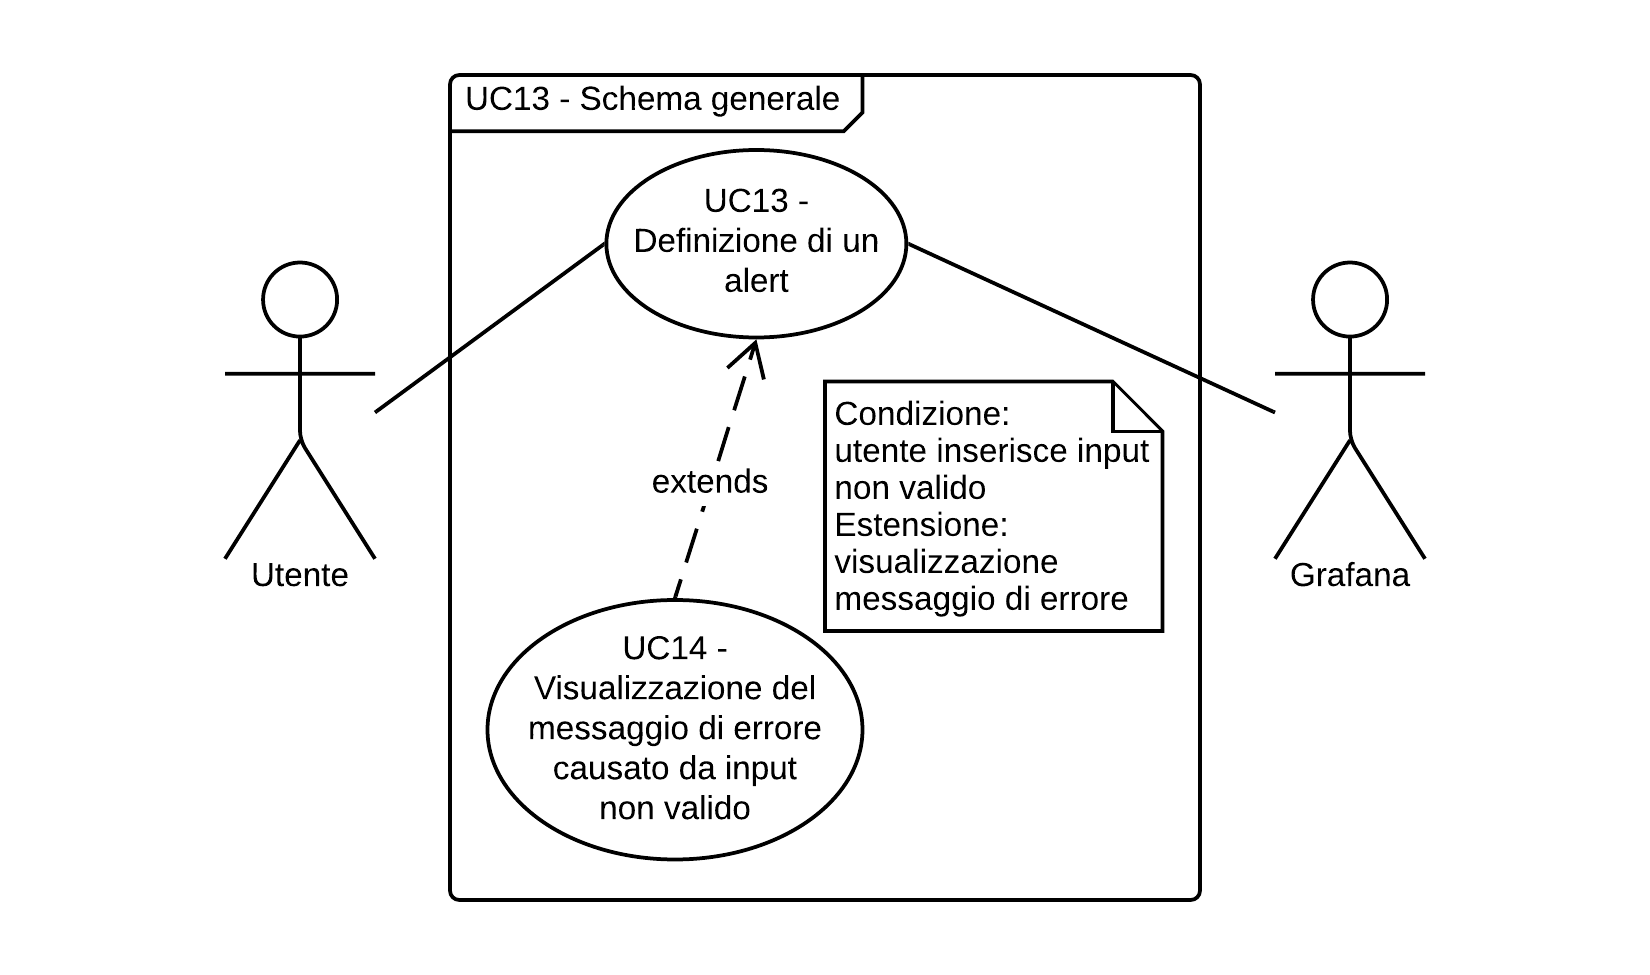
\includegraphics{img/UC13_-_Schema_generale.png}
\caption{Schema generale UC13}
\end{figure}
\subsection{UC13 - Definizione di un alert}
\begin{figure}[H]
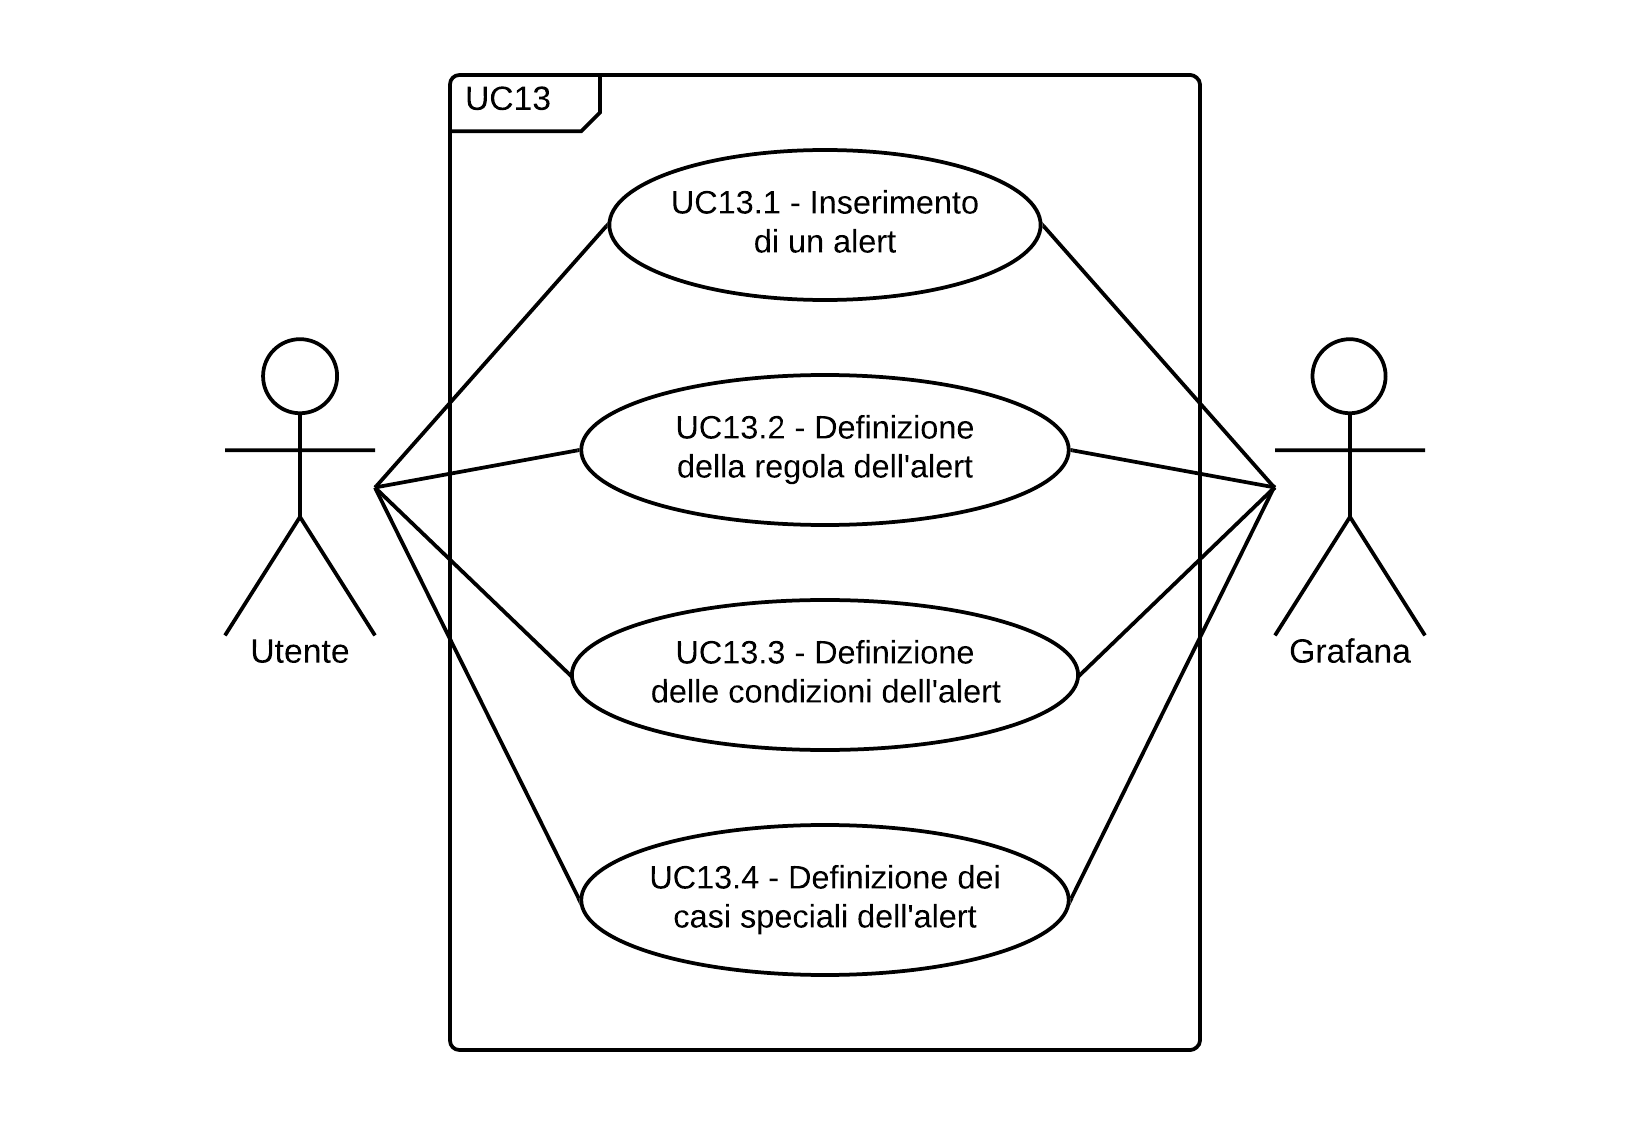
\includegraphics{img/UC13_-_Definizione_di_un_alert.png}
\caption{Diagramma degli use case di UC13}
\end{figure}
\begin{itemize}
	\item \textbf{Codice identificativo}: UC13;
	\item \textbf{Titolo}: Definizione di un alert\glo;
	\item \textbf{Attore primario}: Utente;
	\item \textbf{Attore secondario}: Grafana\glo;
	\item \textbf{Descrizione}: Questo caso d'uso descrive la funzionalità offerta da Grafana\glosp di definire alert\glosp sulle serie di dati che monitora;
	\item \textbf{Precondizione}: L'utente è autenticato nel sistema software Grafana\glosp ed è presente una istanza di Grafana\glosp cloud o locale su cui è stato aggiunto un pannello grafico che monitora una serie di dati;
	\item \textbf{Postcondizione}: Viene inserito e definito con successo un alert\glosp nel pannello grafico scelto;
	\item \textbf{Scenario principale}: 
	\begin{enumerate}
		\item Inserimento di un alert\glosp (UC13.1);
		\item Definizione della regola dell'alert\glosp (UC13.2);
		\item Definizione delle condizioni dell'alert\glosp (UC13.3);
		\item Definizione dei casi speciali dell'alert\glosp (UC13.4).
	\end{enumerate}

	\item \textbf{Estensioni}:	
	\begin{enumerate}
		\item Visualizzazione del messaggio di errore causato da input non valido (UC13).
	\end{enumerate}
\end{itemize}

\subsubsection{UC13.1 - Inserimento di un alert}
\begin{itemize}
	\item \textbf{Codice identificativo}: UC13.1;
	\item \textbf{Titolo}: Inserimento di un alert\glo;
	\item \textbf{Attore primario}: Utente;
	\item \textbf{Attore secondario}: Grafana\glo;
	\item \textbf{Descrizione}: Grafana\glosp fornisce all'utente un modo per inserire alert\glosp sui pannelli grafici;
	\item \textbf{Precondizione}: L'utente deve aver inserito in una dashboard\glosp un pannello grafico;
	\item \textbf{Postcondizione}: Il pannello grafico possiede ora un alert\glo;
	\item \textbf{Scenario principale}: L'utente inserisce in un pannello grafico un alert\glo.
\end{itemize}

\subsubsection{UC13.2 - Definizione della regola di un alert}
\begin{itemize}
	\item \textbf{Codice identificativo}: UC13.2;
	\item \textbf{Titolo}: Definizione della regola dell'alert\glo;
	\item \textbf{Attore primario}: Utente;
	\item \textbf{Attore secondario}: Grafana\glo;
	\item \textbf{Descrizione}: Dopo aver aggiunto un alert\glosp ad un pannello grafico l'utente ha la possibilità di definire la sua regola principale di funzionamento;
	\item \textbf{Precondizione}: L'utente ha aggiunto un alert\glosp al pannello grafico;
	\item \textbf{Postcondizione}: L'utente tramite le funzioni offerte da Grafana\glosp ha definito la regola dell'alert\glosp precedentemente aggiunto;
	\item \textbf{Scenario principale}: L'utente definisce le regole di funzionamento dell'alert\glosp appena inserito, usando le funzioni previste da Grafana\glosp ed inserendo quindi nome e tempi di interrogazione.
\end{itemize}

\subsubsection{UC13.3 - Definizione delle condizioni di un alert}
\begin{itemize}
	\item \textbf{Codice identificativo}: UC13.3;
	\item \textbf{Titolo}: Definizione delle condizioni dell'alert\glo;
	\item \textbf{Attore primario}: Utente;
	\item \textbf{Attore secondario}: Grafana\glo;
	\item \textbf{Descrizione}: Dopo aver aggiunto un alert\glosp ad un pannello grafico l'utente ha la possibilità di definire le sue condizioni di funzionamento;
	\item \textbf{Precondizione}: L'utente ha aggiunto un alert\glosp al pannello grafico;
	\item \textbf{Postcondizione}: L'utente tramite le funzioni offerte da Grafana\glosp ha definito una o più condizioni dell'alert\glosp precedentemente aggiunto;
	\item \textbf{Scenario principale}: L'utente definisce la condizioni di funzionamento dell'alert\glosp appena inserito, usando le funzioni previste da Grafana\glosp e selezionando quindi la funzione di aggregazione dati ed il valore soglia che attiva l'allarme.
\end{itemize}

\subsubsection{UC13.4 - Definizione dei casi speciali di un alert}
	\begin{itemize}
	\item \textbf{Codice identificativo}: UC13.4;
	\item \textbf{Titolo}: Definizione dei casi speciali dell'alert\glo;
	\item \textbf{Attore primario}: Utente;
	\item \textbf{Attore secondario}: Grafana\glo;
	\item \textbf{Descrizione}: Dopo aver aggiunto un alert\glosp ad un pannello grafico l'utente ha la possibilità di definire il suo comportamento al verificarsi di casi particolari;
	\item \textbf{Precondizione}: L'utente ha aggiunto un alert\glosp al pannello grafico;
	\item \textbf{Postcondizione}: L'utente, tramite le funzioni offerte da Grafana\glosp, ha definito uno o più comportamenti speciali dell'alert\glosp precedentemente aggiunto;
	\item \textbf{Scenario principale}: L'utente definisce i comportamenti speciali dell'alert\glosp nei casi particolari come assenza di dati o errori di esecuzione. Per farlo utilizza le funzioni previste da Grafana\glosp selezionando quindi i comportamenti desiderati.
\end{itemize} 